\documentclass[onecolumn, 11pt, a4paper]{article}
\usepackage[a4paper, left = 1cm,right = 1cm, top = 1cm, bottom = 1cm, footskip = 0.5cm]{geometry}
\usepackage{amsmath}
\usepackage{graphicx}
\usepackage{subfig}
\usepackage{float}
\usepackage{wrapfig}
\usepackage{lipsum}
\usepackage[style = numeric, sorting = none]{biblatex}
 
\addbibresource{refs.bib}

\graphicspath{{./images/}}
% \pgfplotsset{compat = 1.17}

% \titlespacing\section{0pt}{12pt plus 4pt minus 2pt}{0pt plus 2pt minus 2pt}
% \titlespacing\subsection{0pt}{12pt plus 4pt minus 2pt}{0pt plus 2pt minus 2pt}

\author{
  % George Herbert\\
  % \texttt{cj19328@bristol.ac.uk}
}
\date{}

\title{\vspace{-2em}No Entry Sign Challenge Report\vspace{-2em}}

\begin{document}

\maketitle

% \begin{abstract}
%     Abstract
% \end{abstract}

\section{The Viola-Jones object detector}

\subsection{Ground truth and visualisation}

\begin{figure}[H]
  \vspace{-2em}
  \centering
  \subfloat[NoEntry1.jpg]{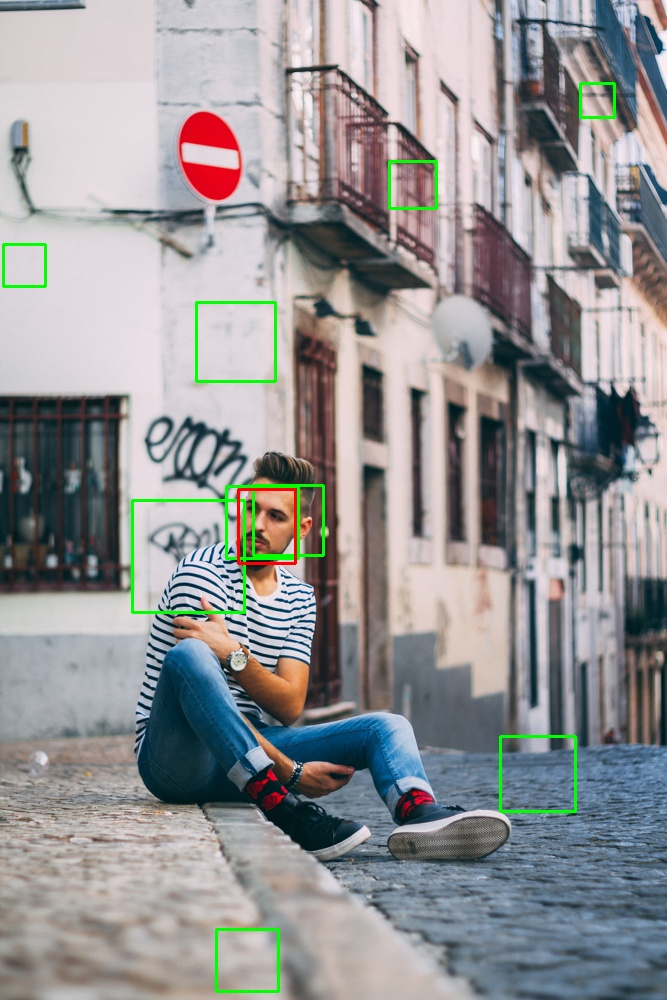
\includegraphics[height = 0.18\textheight]{images/NoEntry1.jpg}\label{fig:face1}}
  \hfill
  \subfloat[NoEntry5.jpg]{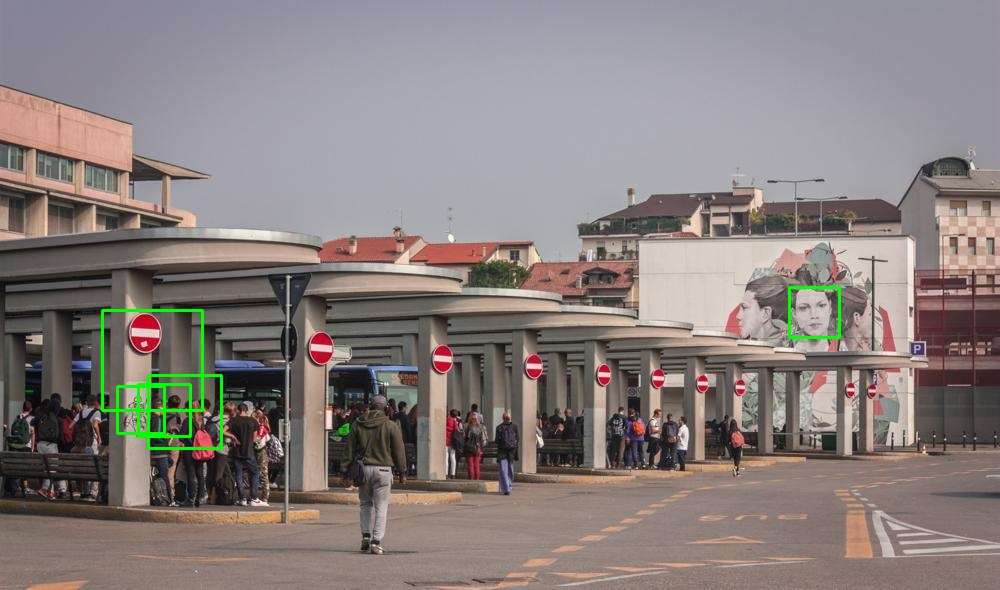
\includegraphics[height = 0.18\textheight]{images/NoEntry5.jpg}\label{fig:face5}}
  \hfill
  \subfloat[NoEntry11.jpg]{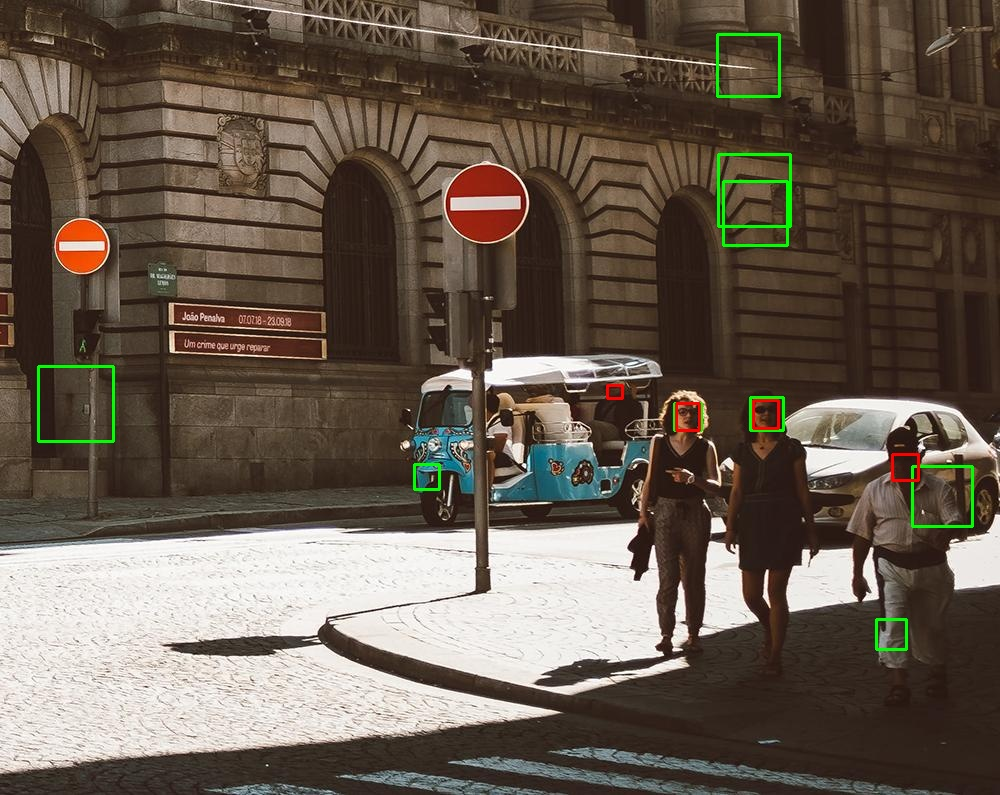
\includegraphics[height = 0.18\textheight]{images/NoEntry11.jpg}\label{fig:face11}}
  \hfill
  \subfloat[NoEntry2.jpg]{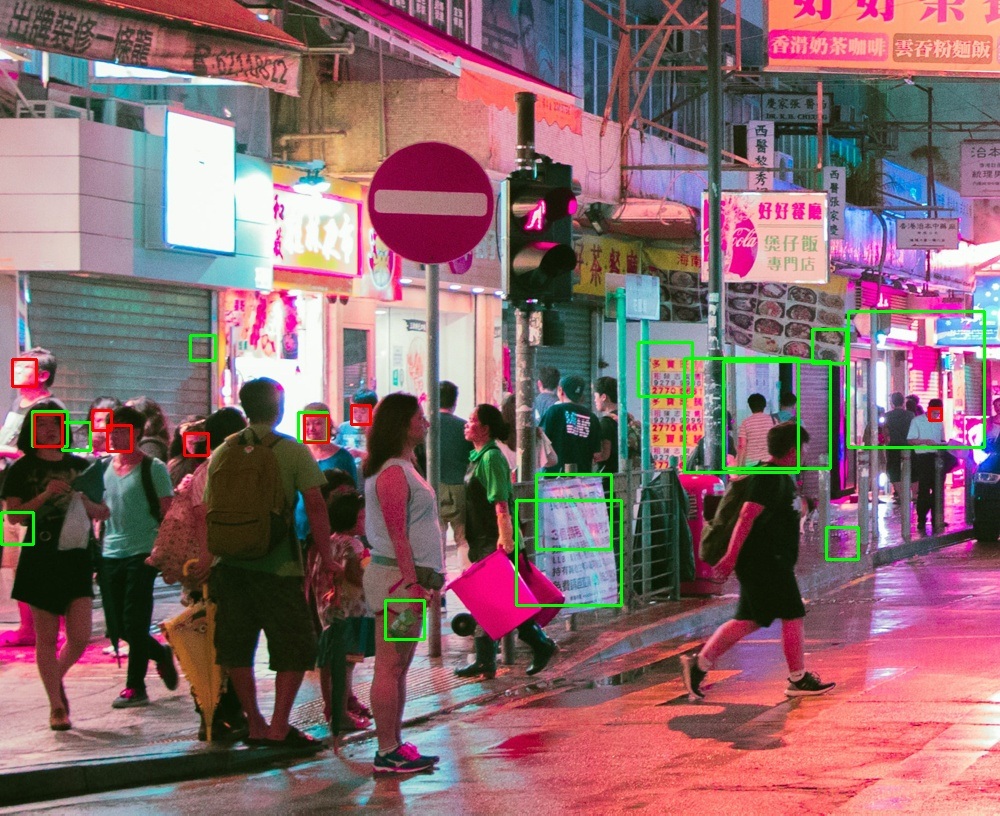
\includegraphics[height = 0.17\textheight]{images/NoEntry2.jpg}\label{fig:face2}}
  \hfill
  \subfloat[NoEntry4.jpg]{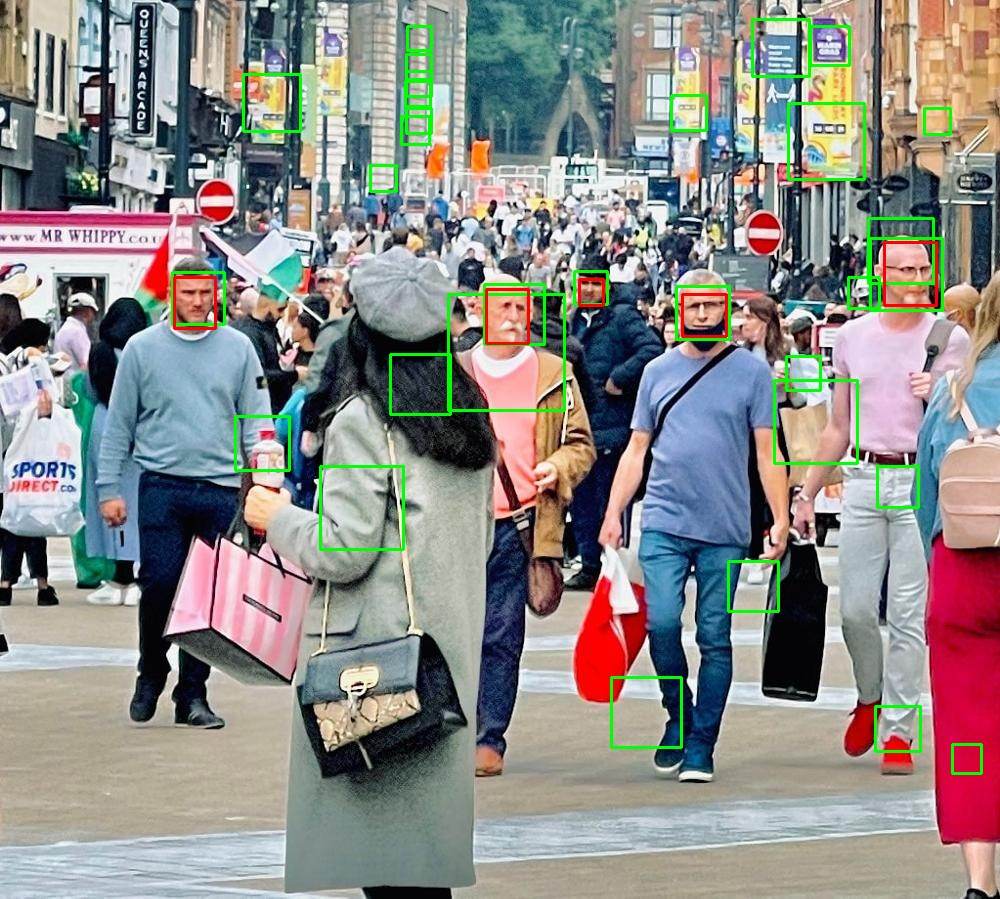
\includegraphics[height = 0.17\textheight]{images/NoEntry4.jpg}\label{fig:face4}}
  \hfill
  \subfloat[NoEntry7.jpg]{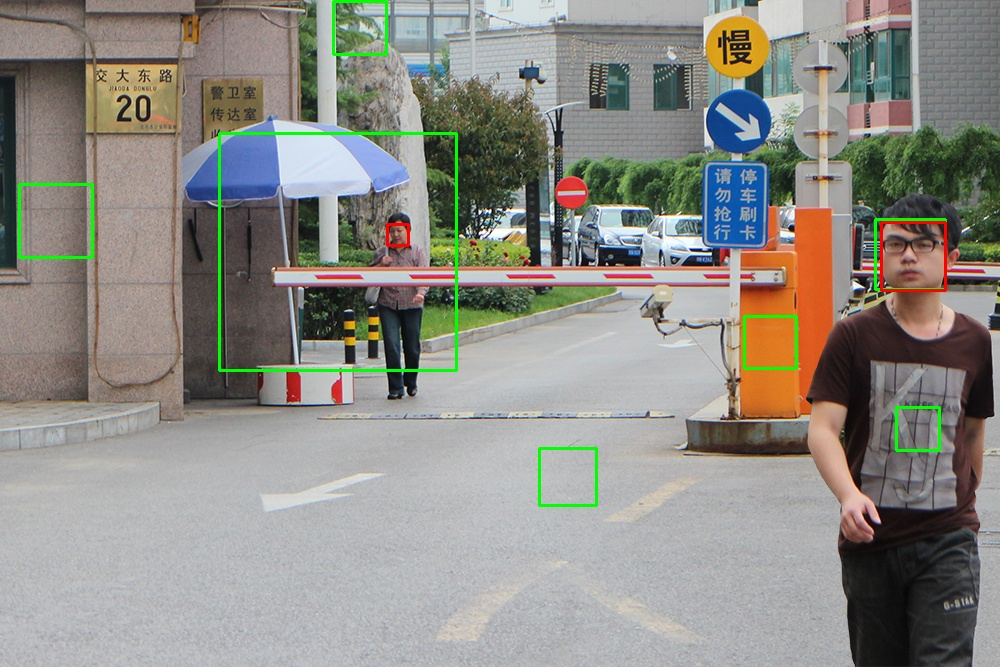
\includegraphics[height = 0.17\textheight]{images/NoEntry7.jpg}\label{fig:face7}}
  \caption{Six images with the bounding boxes of the ground truths (in red) and actually detected instances (in green) from the frontal face detector}\label{fig:face}
\end{figure}

\subsection{Intersection-over-union, true positve rate and F\textsubscript{1} score}

\begin{wraptable}{r}{0.4\textwidth}
  \vspace{-2.5em}
  \begin{center}
  \caption{TPR and F\textsubscript{1} score of the frontal face detector on each image}\label{tab:face}
  \begin{tabular}{l l l} 
    \hline\hline
    Image & TPR & F\textsubscript{1} score\\
    \hline
    NoEntry0.jpg & Undefined & 0.00 \\ 
    NoEntry1.jpg & 1.00 & 0.20 \\ 
    NoEntry2.jpg & 0.25 & 0.18 \\ 
    NoEntry3.jpg & Undefined & Undefined \\ 
    NoEntry4.jpg & 1.00 & 0.28 \\ 
    NoEntry5.jpg & Undefined & 0.00 \\ 
    NoEntry6.jpg & Undefined & 0.00 \\ 
    NoEntry7.jpg & 0.50 & 0.22 \\ 
    NoEntry8.jpg & Undefined & 0.00 \\ 
    NoEntry9.jpg & Undefined & 0.00 \\ 
    NoEntry10.jpg & Undefined & 0.00 \\ 
    NoEntry11.jpg & 0.50 & 0.31 \\ 
    NoEntry12.jpg & 0.00 & 0.00 \\ 
    NoEntry13.jpg & Undefined & 0.00 \\ 
    NoEntry14.jpg & Undefined & 0.00 \\ 
    NoEntry15.jpg & Undefined & 0.00 \\ 
    \hline
  \end{tabular}
  \end{center}
\end{wraptable} 

In an object detection task, the true positive rate (TPR) is the probability that an object will be positively detected.
However, the first practical difficulty that arises in calculating the TPR is whether or not to define a predicted bounding box as a being a true positive or a false positive.
I opted to define a detected bounding box as being a true positive if it had an intersection-over-union (IoU) value greater than 0.5 with a ground truth bounding box, as this is considered a good score \cite{iou}.
Moreover, for each ground truth bounding box, I only defined the detected bounding box with the largest IoU value as being a true positive if there was more than one intersecting detected bounding box.

In any detection task, TPR can be a flawed metric to use to define how well a given model performs.
This is because, it is possible to achieve a TPR of 100\% by detecting every possible pixel region as being the object being detected, despite having a large number of false positives.
As a result of this, the F\textsubscript{1} score is often used as a measure of a model's accuracy.
F\textsubscript{1} score is the harmonic mean of sensitivity (i.e. TPR) and precision.
Table \ref{tab:face} displays the F\textsubscript{1} score and TPR that `face.cpp' achieved on each of the NoEntry\textasteriskcentered.jpg images

\clearpage

\section{Building and testing my own detector}

\subsection{Training performance}

ROC graph
% \begin{tikzpicture}
% \begin{axis}[]
% \addplot+[
%   only marks,
%   % mark size=2.9pt
% ]
% table[]
% {fpr_tpr.dat};
% \end{axis}
% \end{tikzpicture}

\subsection{Testing performance}

\section{Integration with shape detectors}

\section{Improving my detector}



\clearpage

\printbibliography
    

\end{document}